\chapter{Opis tabel}
\label{chap:opistabel}

\begin{figure}[ht!]
\centering
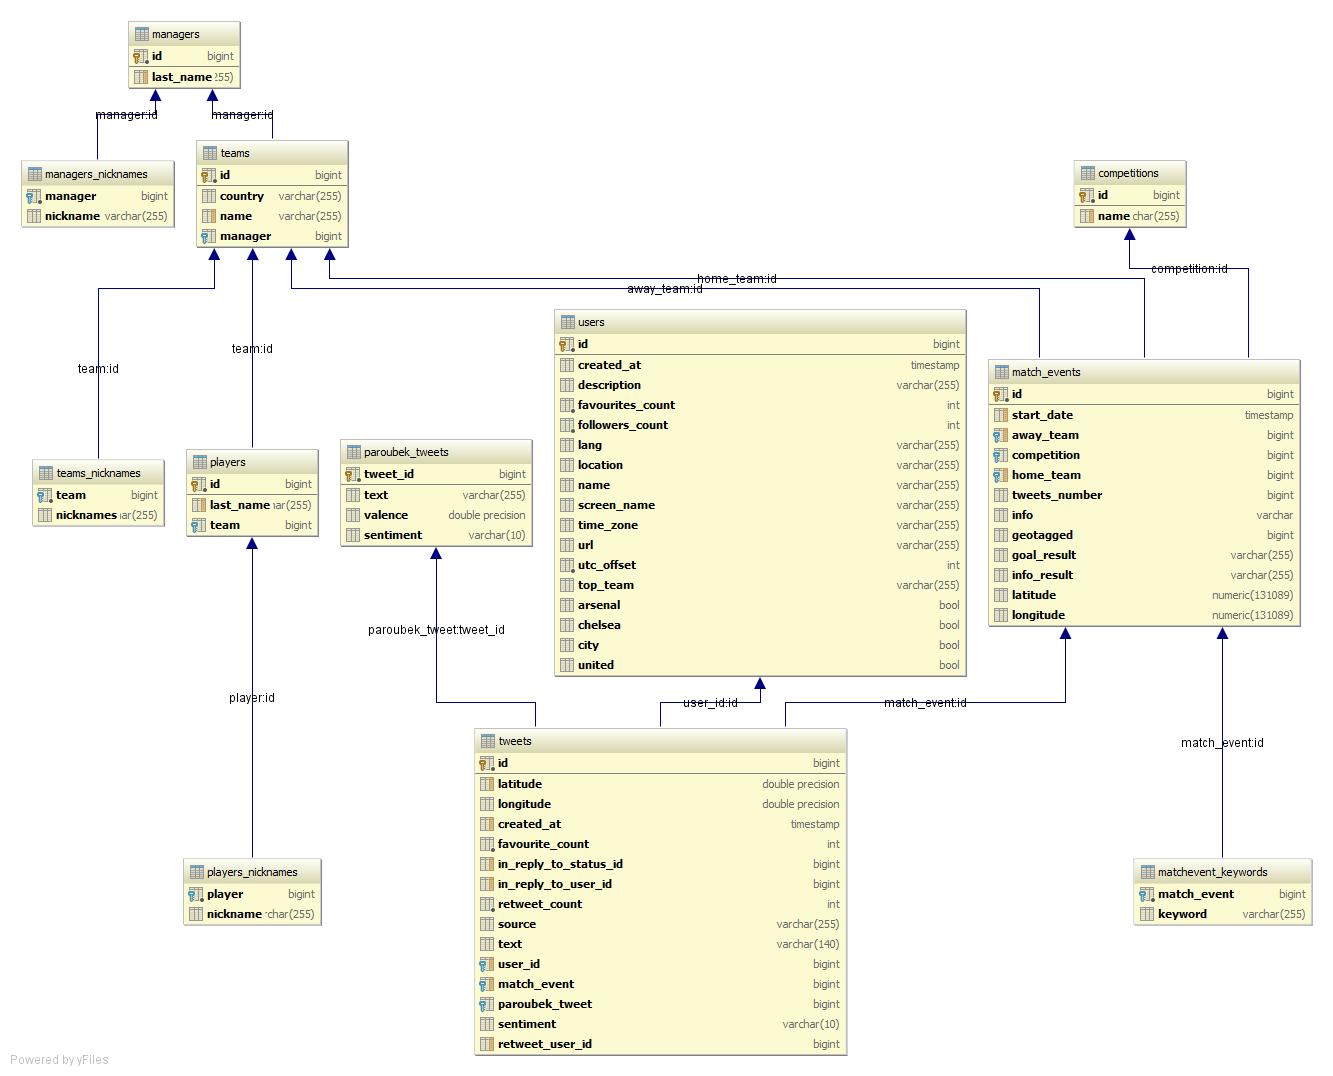
\includegraphics[width=160mm]{img/db-schema-intellij.png}
\caption{Schemat bazy danych}
\label{image:schemat-bazy-dodatek}
\end{figure}

\begin{description}
\item[competitions] rodzaje rozgrywek, w których brały udział drużyny \\
\textit{id} -- identyfikator wiersza \\
\textit{name} -- nazwa rozgrywek (np. Champions League, Liga Angielska)

\item[managers] nazwiska menadżerów (trenerów) drużyn \\
\textit{id} -- identyfikator wiersza \\
\textit{last\_name} -- nazwisko menadżera

\item[managers\_nicknames] popularne określenia, przezwiska menadżerów drużyn \\
\textit{manager} -- klucz obcy wskazujący rekord w tabeli \textit{managers} \\
\textit{nickname} -- dodatkowe określenie menadżera

\item[match\_events] nasłuchiwane spotkania między drużynami \\ 
\textit{id} -- identyfikator wiersza \\ 
\textit{start\_date} -- data rozpoczęcia spotkania \\
\textit{away\_team} -- identyfikator drużyny gości; klucz obcy do tabeli
\textit{teams}\\
\textit{competition} -- identyfikator rozgrywek; klucz obcy do tabeli
\textit{competitions}\\
\textit{home\_team} -- identyfikator drużyny gospodarzy; klucz obcy do tabeli
\textit{teams}\\
\textit{tweets\_number} -- liczba tweetów zebranych dla spotkania\\
\textit{info} -- krótki opis spotkania wraz z wynikiem\\
\textit{geotagged} -- liczba tweetów z geolokalizacją dla spotkania\\
\textit{goal\_result} -- wynik meczu\\
\textit{info\_result} -- krótki opis spotkania wraz z wynikiem\\
\textit{latitude} -- szerokość geograficzna miejsca meczu (stadionu)\\
\textit{longitude} --  długość geograficzna miejsca meczu (stadionu)


\item[matchevent\_keywords] dodatkowe słowa kluczowe dla meczów (np. nazwa
stadionu, nazwisko sędziego, etc.) \\
\textit{matchevent} -- klucz obcy wskazujący rekord w tabeli
\textit{match\_events} \\
\textit{keyword} -- słowo kluczowe

\item[paroubek\_tweets] wyniki wyliczania sentymentu tweetów \\
\textit{tweet\_id} -- identyfikator tweeta; klucz obcy do tabeli
\textit{tweets}\\
\textit{text} -- oczyszczony tekst tweeta\\
\textit{valence} -- wartość \textit{valence} \rref{subsubsection:pakandparoubek} algorytmu określania
sentymentu\\

\item[players] zawodnicy drużyn \\
\textit{id} -- identyfikator wiersza \\
\textit{last\_name} -- nazwisko zawodnika\\
\textit{team} -- identyfikator drużyny zawodnika; klucz obcy do tabeli \textit{teams}\\
 
\item[players\_nicknames] popularne przezwiska, określenia piłkarzy\\
\textit{player} -- identyfikator piłkarza; klucz obcy do tabeli \textit{players}\\
\textit{nickname} -- określenie piłkarza\\
 
\item[teams] nasłuchiwane drużyny\\
\textit{id} -- identyfikator wiersza \\
\textit{country} -- kraj drużyny\\
\textit{name} -- nazwa klubu\\
\textit{manager} -- identyfikator menadżera; klucz obcy do tabeli
\textit{managers}\\
 
\item[teams\_nicknames] popularne przezwiska, określenia drużyn\\
\textit{team} -- identyfikator drużyny; klucz obcy do tabeli \textit{teams}\\
\textit{nicknames} -- określenie drużyny\\
 
\item[tweets] zebrane tweety\\
\textit{id} -- identyfikator wiersza \\
\textit{latitude} -- szerokość geograficzna wysłania tweeta\\
\textit{longitude} -- długość geograficzna wysłania tweeta\\
\textit{created\_at} -- data utworzenia tweeta\\
\textit{favourite\_count} -- liczba osób, które oznaczyły tweet jako ulubiony\\
\textit{in\_reply\_to\_status\_id} -- identyfikator tweeta, na który ten wpis
jest odpowiedzią\\
\textit{in\_reply\_to\_user\_id} -- identyfikator użytkownika, na którego
tweeta ten wpis jest odpowiedzią\\
\textit{retweet\_count} -- liczba osób, które przekazały ten tweet dalej
\ang{retweet}\\
\textit{source} -- źrodło wysłania tweeta (nazwa aplikacji)\\
\textit{text} -- tekst tweeta\\
\textit{user\_id} -- identyfikator autora wpisu; klucz obcy do tabeli
\textit{users}\\
\textit{match\_event} -- identyfikator spotkania, którego wpis dotyczy; klucz
obcy do tabeli \textit{match\_events}\\
\textit{paroubek\_tweet} -- identyfikator do rekordu z obliczoną wartością
sentymentu (pokrywa się z kolumną \textit{id} tej tabeli); klucz obcy do tabeli
\textit{paroubek\_tweet}\\
\textit{sentiment} -- tekstowe określenie sentymentu tweeta, np. \textit{POS}
(pozytywny), \textit{NEG} (negatywny), \textit{NEU} (neturalny)\\
\textit{retweet\_user\_id} -- identyfikator użytkownika, którego tweet został
podany dalej jako ten wpis\\
 
\item[users] użytkownicy Twittera będący autorami zebranych tweetów\\
\textit{id} -- identyfikator wiersza \\
\textit{created\_at} -- data rejestracji użytkownika\\
\textit{description} -- opis użytkownika w serwisie Twitter\\
\textit{favourites\_count} -- liczba osób, którego oznaczyły danego
użytkownika jako ulubionego\\
\textit{followers\_count} -- liczba osób śledzących\\
\textit{lang} -- główny język użytkownika\\
\textit{location} -- miejsce przebywania użytkownika (wpisywane ręcznie przez
użytkownika)\\
\textit{name} -- nazwa użytkownika\\
\textit{screen\_name} -- wyświetlana nazwa użytkownika\\
\textit{time\_zone} -- strefa czasowa użytkownika\\
\textit{url} -- adres strony profilowej użytkownika w serwisie Twitter\\
\textit{utc\_offset} -- różnica czasu między strefą czasową użytkownika a
czasem UTC (ang. \textit{Coordinated Universal Time} -- uniwersalny czas
koordynowany)\\
\textit{top\_team} -- drużyna, której mecze użytkownik komentował najczęściej;
klucz obcy do tabeli \textit{teams}\\
\textit{arsenal} -- oznaczenie czy użytkownik jest zwolennikiem, czy
przeciwnikiem Arsenalu \rref{subsubsection:wykrywaniezwolennikow} \\ 
\textit{chelsea} -- oznaczenie czy użytkownik jest zwolennikiem, czy
przeciwnikiem Chelsea \\
\textit{city} -- oznaczenie czy użytkownik jest zwolennikiem, czy
przeciwnikiem Manchesteru City\\
\textit{united} -- oznaczenie czy użytkownik jest zwolennikiem, czy
przeciwnikiem Manchesteru United
\end{description}